\section{The mean teacher approach to semi supervised learning}
\label{sec:mean_teacher}

As mentioned multiple times already, the starting hurdle for building machine learning solutions is obtaining enough high quality annotated data. 
For image segmentation tasks, this means segmentation masks, which are notoriously time consuming to produce. 
In our case, no annotated data was present in the beginning and it would be unreasonable to spend a large amount of time to annotate a lot of images, so only a limited amount of labeled samples were produced. 
In contrast, unlabeled images can be obtained very quickly and in large amounts, as one good measurement run can produce hundreds to thousands of images (even though not all of them may be usable).

Thus it would be very beneficial if we could make use of this unlabeled data in some way during training. 
Approaches to learning that utilize both labeled and unlabeled data are called \emph{semi-supervised learning}, in contrast to \emph{(fully-)supervised} or \emph{unsupervised learning}, where only labeled or no labeled data is used respectively. 
One example for such a procedure is called the \emph{Mean Teacher approach}.\cite{tarvainenMeanTeachersAre2018}

The main idea of the Mean Teacher approach it to use two models, one \emph{student} and one \emph{teacher}, and have the student learn from examples produced by the teacher.

The reason unlabeled data is not directly usable for model training is that no classification cost can be applied to the outputs, as the target is undefined.
While there is no way to automatically generate a 100\% accurate target, as this is essentially what we try to train our model to do, when we look at it the other way around, we can use a model to approximate the target to a degree.
However, using the same model we want to train to simply approximate its own training samples would not provide any benefit.
Two steps are are used in the Mean Teacher method to still make use of these kinds of \emph{pseudolabels}.

As mentioned in \ref{sec:training}, augmentation and regularization techniques have the purpose of enabling the model to learn the concept of its target function more broadly, since small variances in the input should still produce a similar output. 
This can be applied not only when comparing the output of the model to the ground truth, but also when comparing the outputs of the model for the same input data, but different levels of noise. 
In a sense, if the model has properly learned the correct abstractions, its prediction should be similar, even if the input is slightly different.
What this means concreetly in this case, is that the method uses the teacher to make a prediction on an input without any noise and then computes student predicitons on the same input to which  augmentations have been applied.
In general, the teacher should have an easier time to predict accurate labels for a sample without noise, so a slightly better approximation of the theoretical correct labels should be produced. 
A \emph{consistency cost} can then be applied between student and teacher predictions which are then used in the same way as the \emph{classification cost} to update student weights.

Another way to improve the relative quality of the pseudolabels is to improve the teacher model they are generated by.
This is where the second key concept of the method comes in.
Instead of using the same weigths for both student and teacher models, the \emph{exponential moving average} (EMA) of the student weights are used for the teacher.
What this means is, if $\theta_t$ are the weights of the student at step $t$ and $\theta'_t$ are teacher weights at the same point, $\theta'_{t+1}$ is defined as follows:
$$
    \theta'_{t + 1} = \alpha\theta'_t + (1 - \alpha) \theta_t
$$
where $\alpha$ is a smoothing coefficient called the \emph{EMA decay}.

The EMA of a model has been observed to be slightly better than the model itself, as well as being more stable during the training process, since changes to the student model are only adapted slowly. Combining this with the noisy student inputs makes it possible to extract a lot of improvment from unlabeled examples, but can also be applied during training steps with labeled data. 

\begin{figure}[htbp]
   \makebox[\textwidth][c]{
        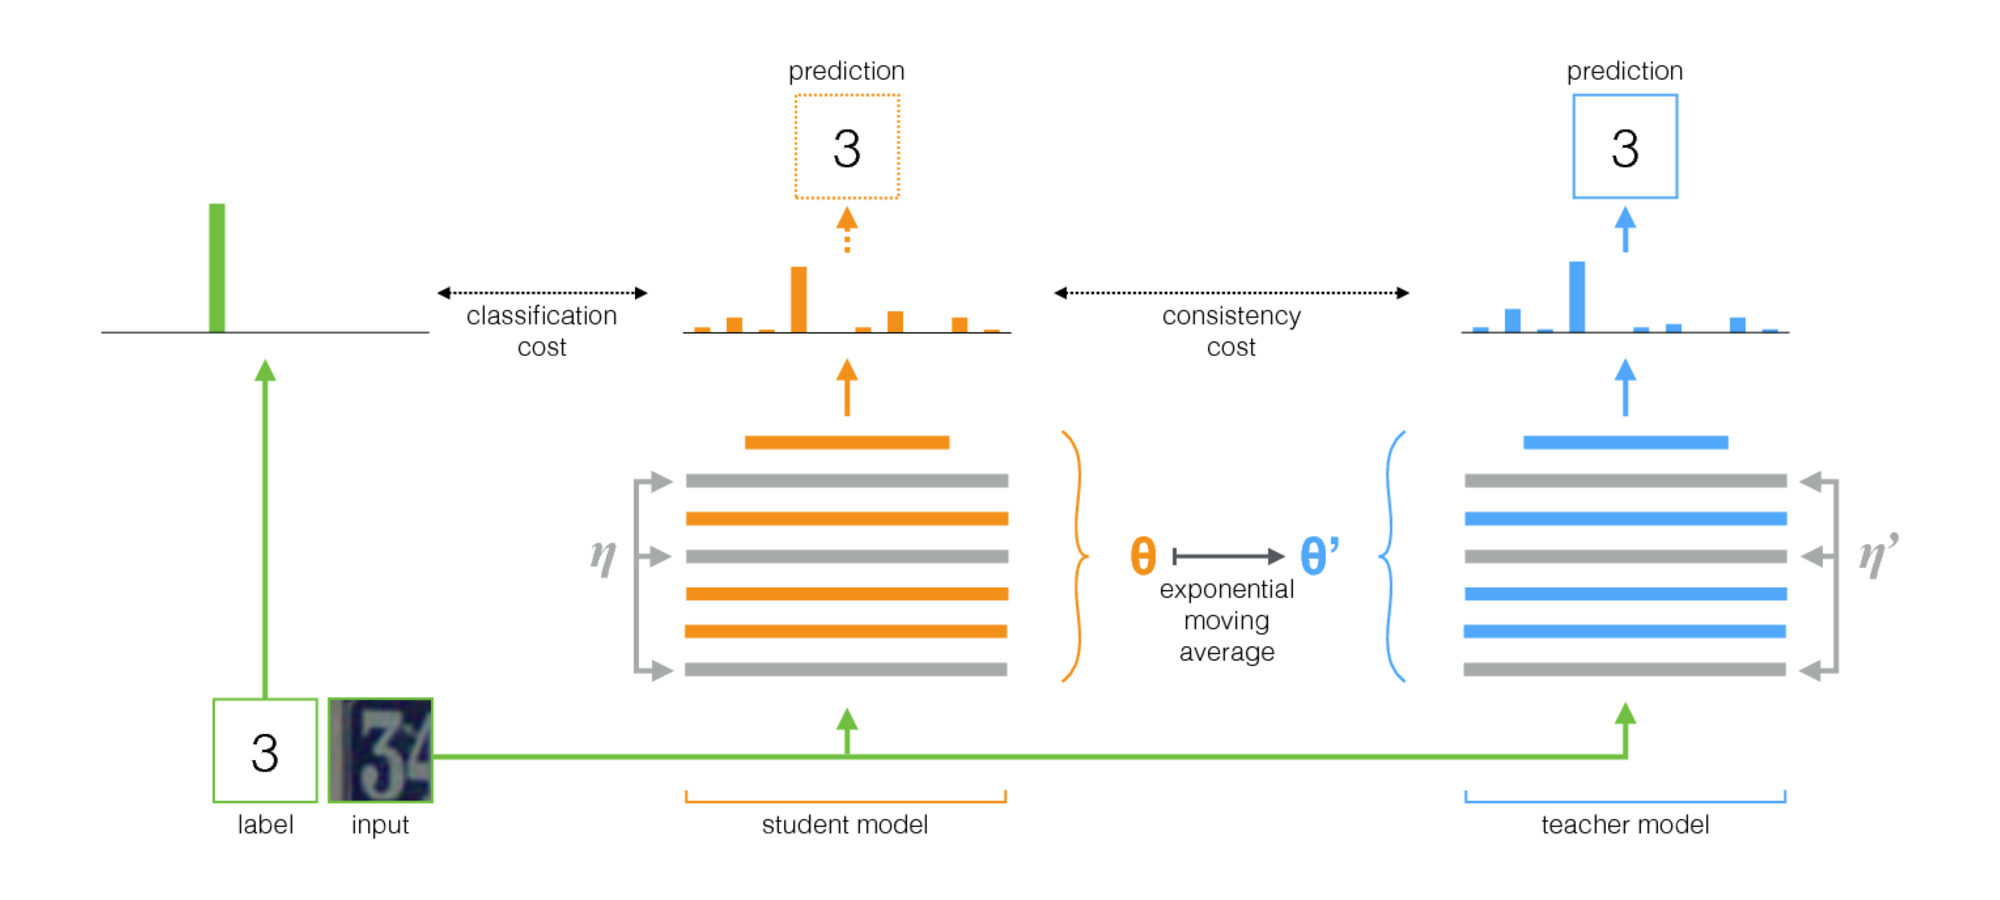
\includegraphics[width=\textwidth]{images/mean_teacher.png}
   }
   \caption{Schematic depiction of the Mean Teacher method. The graphic illustrates a single training step with one labeled sample for the image classification task. The classification loss is applied between the ground truth and the model predictions, while the consistency cost is computed between the soft outputs of both models. After updating the student weights, new teacher weights are computed as the EMA of the student weights. Steps with unlabeled samples simply omit the classification cost. Image taken from \cite{tarvainenMeanTeachersAre2018}}
   \label{fig:mean_teacher}
\end{figure}

During traing, it is necessary to apply a relative weight between classification loss and consistency loss, since initially, the teacher model may produce very bad outputs and which might also differ a lot from the student outputs, since no concepts haven been learned yet. 
If the consistency is given too much weight the model will prioritize being consistent with the teacher over predicting the correct classes for the labeled examples, potentially hurting or preventing any training progress. 
Thus, the weight of the consistency loss should start low and be slowly ramped up over the period of the training. 

Another key aspect of the method is considering which augmentations are chosen for the student inputs. To produce a large enough difference between outputs, strong augmentations are necessary to achieve the best improvements. The augmentations should also be well tailored to the dataset that is being trained on. 

Lastly, as mentioned above, the method introduces the hyperparameter $\alpha$ into the training, which has a big influence over the improvement that can be achieved. If it is too low, the benefits of using the EMA may not be present as much, since the teacher is too similar to the student. If it is too high, the teacher may not be updated quickly enough to incorporate the students improvement. 

The applicability of the mean teacher method will be more closely examined during the experiments of the thesis, with the goal to improve overall accuracy as well as generalization of the model produced. 